\section*{Metod}
När en spelplan är given så delas denna in i domäner i form av rektanglar. De kan vara olika stora och ha olika mått. Detta illustreras i den övre delen av figur 1. 
\newline
\newline
\begin{minipage}{\linewidth}
\begin{center}
    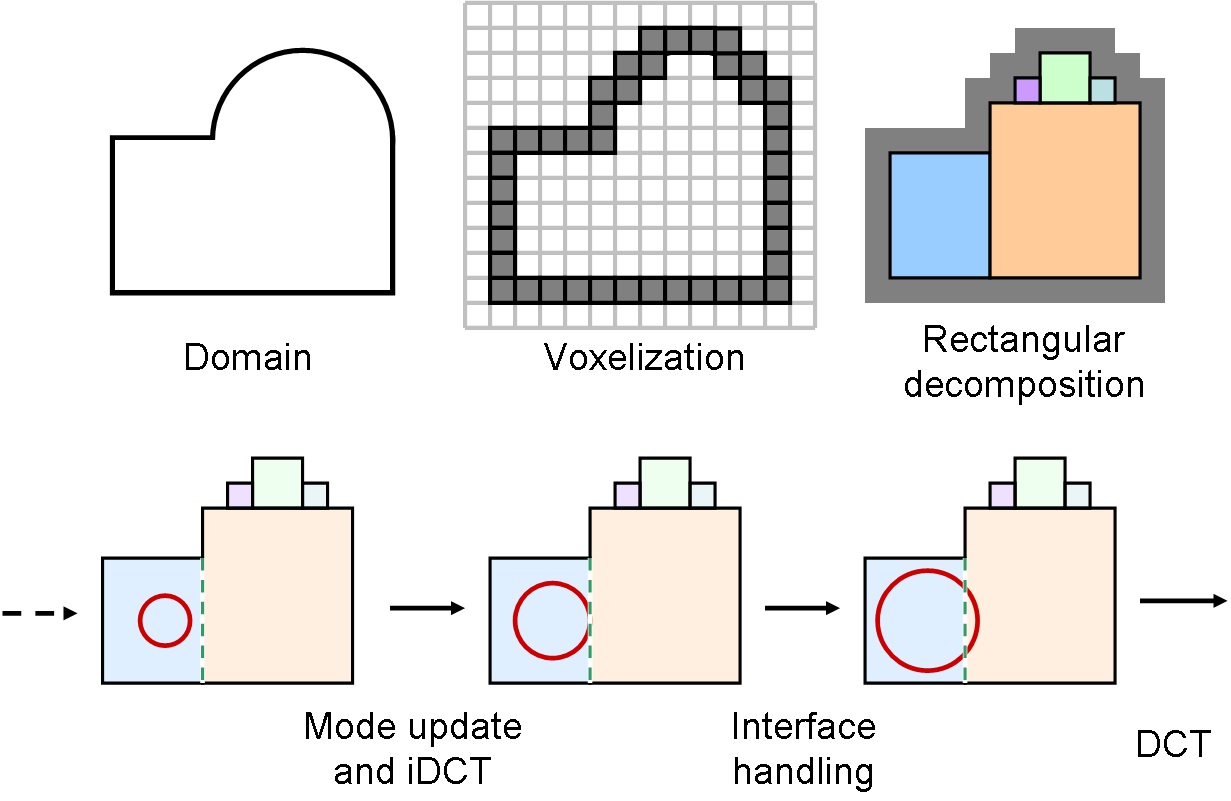
\includegraphics[width = 0.5\linewidth]{domain.jpg}\\*
    \caption{Figur 1. Domänen delas upp i rektanglar\cite{rect_decomp}.}\\*
    \end{center}
\end{minipage}
\newline
\newline
För att våran metod ska kunna behandla absorberande randvillkor spektralt måste vi först utveckla den för inhomogena randvillkor. Standardmetoden för att angripa inhomogena randvillkor är att dela upp vågfunktionen $u$,
\begin{equation}
u(x,t) = q(x,t) + w(x,t),
\end{equation}
där $q$ är en $[0,L]$-periodisk del som uppfyller vågekvationen med homogena randvillkor och en del $w$, känd för alla tider och positioner, som uppfyller de inhomogena randvillkoren. Nu kan vågekvationen skrivas upp för den periodiska delen $q$ med en källterm endast beroende utav $u$
\begin{equation} \label{eq:abcstep}
q_{tt} - v^{2}q_{xx} = \left(\frac{(L-x)^{2}}{2L}\right)(u_{t})_{xx}(0,t) - \left(\frac{x^{2}}{2L}\right)(u_{t})_{xx}(L,t) + \left(\frac{v^{2}}{L}\right)[u_{t}(L,t) - u_{t}(0,t)].
\end{equation}
Då $w$ är känt i varje steg och $q$ är periodisk över $[0,L]$ kan vi använda Discrete Cosine Transform för att uppdatera det inre av våra rektanglar.\\*
Sedan kommunicerar rektanglarna med varandra för att vågen skall kunna propagera mellan domänerna, illustrerat i den nedre delen av figur 1.

